\chapter{Literature review} 
\label{Literature Review} 
\lhead{Chapter 2. \emph{Literature Review}} 

One of the classic questions in the philosophy of cognition is - What is the relationship between perception and action? One of the dominant ideas is that the purpose of perception is to gather information for guiding action, while action is a means to acquire perceptual information regarding the environment. In reaching action, action is directed towards objects of interest in the external environment. The body is central to the process of reaching action. Not only is the reach carried out by bodily movements, but the targets of reaching actions also lie in space close to the body(peri-personal space). Thus, for a reaching action, the cognitive system of the agent requires i) knowledge of body for computing the state of the effector (the body entity with which the action is carried out), and ii) information regarding the object of interest (the target entity on which the action is carried upon). Perceptual processes provide knowledge to the system regarding both these entities.

The aim of this chapter is to provide relevant background and discuss key concepts, theories and empirical findings that led to the development of the conjecture that we have investigated in this thesis. This chapter will thus be divided into two parts - the body and the target. Part I consists of a brief discussion on body representation, and its role in motor control. In Part II, we delve into theories and findings regarding peri-personal space, where the reach action target lies, and its implications in unfolding of action. I will end with connecting these distinct strands of literature and stating the conjecture. 


\section{Body representation and Action}

Goal-directed action require information about properties of one's body, in order to plan movements, and guide the action. These properties include both structural and positional parameters of the body. Precise position of one's limbs, not only during action initiation (t = 0), but also during the action execution, is an important parameter for a successful action. Furthermore, information regarding structural properties of one's body, such as body configuration, body size, flexibility of joints, muscle strength, are necessary so that movements do not occur in biologically impossible or painful manner. According to the review by \citeA{ataria2021body}, one of the claims in the literature is that the cognitive system of the agent represents the above mentioned properties in an integrated representation of the body, termed as \emph{body schema}. Importantly, body schema is conceptually distinguished from other body representations like body image, by the notion that the parameters encoded in body schema are in a specific format. Evidence from \citeA{schwoebel2005evidence}'s study suggests that body parameters are encoded in three distinct representational formats - sensorimotor, visuo-spatial, and linguistic. Body schema encodes the bodily parameters in a sensorimotor format, which the motor system can directly exploit.

In the control-theoretic model of action, two types of process models have been proposed- the inverse model and the forward model, both of which function parallelly. The claim is that body schema plays a role in both these processes. The inverse model computes the motor commands required to achieve the goal, or the final state of the action, constrained by the current body capacities, which are represented in the body schema.  The forward model predicts sensorimotor consequences of the action \cite{wolpert2001motor}. Here, the execution of action is guided by matching the anticipatory model of the body, with the current model of the body, as represented by the body schema. \citeA{ataria2021body} thus proposes a dual function of body schema - description of the body at a spatial resolution and format which can be utilized by the motor system, and for the anticipatory control of action.

\subsection{Construction of body schema}

One of the dominant questions regarding the body schema is -  what are the computations underlying the construction of body schema. \citeA{ataria2021body} suggests that construction of body schema is a dynamic process, that is, the body representation is continuously updated to adapt to the bodily changes throughout development and other short term changes like changes in environment, ill-health, pregnancy, or tool use. 

One of the theories for understanding the construction of body schema is that the generation of body schema can be thought of as an inference problem, to compute the most reliable estimates of body parameters from the inflow of sensory inputs from various sensory modalities, like vision and proprioception \cite{van1999integration}. The Bayesian model of multi-sensory integration proposes that the cognitive system computes the most probable output, here, the parameters specifying the body schema, from the sensory cues available, on the basis of the reliability of the sensory cues (noise), and the prior beliefs encoded in the system regarding the relevance of the cues.  In a novel bodily situation, online sensory cues will be favoured, versus the beliefs regarding the past body representations. Furthermore, the success of action also informs the construction of the body schema. If the action is successful, the process underlying the generation of body schema is confirmed, whereas, if the action is unsuccessful, the body schema needs to be updated for future actions. Thus, Bayesian view provides a description of how body schema is dynamically constructed. 

 Furthermore, the role of integration of inputs from multiple modalities in demonstrating the plasticity of the body representation has also been empirically demonstrated through the Rubber Hand Illusion. In this paradigm, when a rubber hand is stroked synchronously with a participant's unseen real hand, they tend to i) perceive the location of their hand as displaced towards the rubber hand \cite{tsakiris2005rubber} , ii) perceive tactile sensation through the rubber hand \cite{pavani2000visual}, and iii) experience a feeling of ownership over the rubber hand \cite{longo2008embodiment}.  

 There are two major challenges regarding the computations of the multi-sensory integration processes underlying the emergence of body schema. The first is how to identify and select which are the relevant sensory signals to bind together- a problem termed as the "parsing problem". The second problem is, once the relevant signals are selected, how are the signals integrated into a coherent body representation? Every sensory signal is encoded in a different modality-specific format, and in a particular frame of reference, which needs to be resolved into a common format and reference frame. Furthermore, different sensory cues are assigned different weights based on their reliability and relevance. How are these weights assigned, is an important question to consider.

Summarizing this section, body schema specifies bodily parameters which are relevant for action planning and control, and the construction of body schema is a dynamic process relying on a process of multi-sensory integration of sensory inputs from vision and proprioception. We will now turn towards a discussion regarding perception of the action target and the representation of its spatial location.

 \section{Peri-personal space}

 \begin{figure}
\centering    
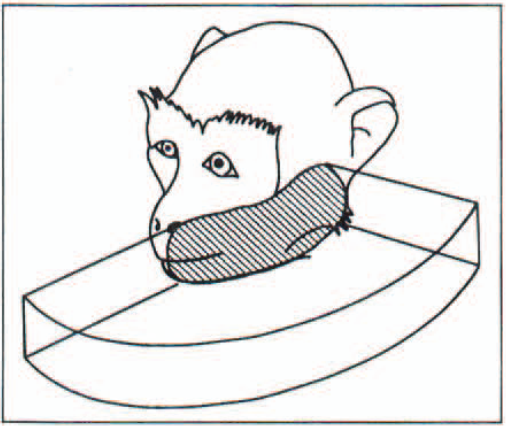
\includegraphics[width=70mm]{Images/bimodal.png}
\caption{Spatially corresponding tactile receptive field (striped) and visual receptive field (boxed) of a bimodal neuron in putamen \citep{graziano1994mapping}}
\label{fig:bimodal}
\end{figure}

 In the cognitive system, the representation of space provides a framework regarding how different objects in the external environment are located with respect to each other, and with respect to the self. Other than abstract and geographical spatial representations, the prominent characteristic of space representation is that body, or a body-part is the origin of spatial representations. Spatial information is processed in several reference frames, depending on the sensory source of the information and the agent environment interaction. For example, the spatial location of an approaching bee will be processed not only in eye-centered and head-centered reference frames due to visual and auditory inputs, but also in reference to the hand to which it is approaching to avoid getting strung \cite{serino2019peripersonal}. However, exponentially, the agent does not have explicit access to these distinct representations, suggesting integration of different reference frames into a unified global reference frame (as reviewed by \citeA{serino2019peripersonal}). 

Peri-personal space is the region of space in close proximity to the body. Its representation is distinct from the representations of extra-personal space (regions of space far from the body), based on findings from lesion studies in monkeys that show that different neuronal populations encode peri-personal and extra-personal space \cite{rizzolatti1983deficits}.

%Peri-personal space is relevant for this work because the target of reach actions lie in the peri-personal space. For the purpose of this thesis, it is thus helpful to think of peri-personal space representations in terms of representing the distance of the object from the part of body in its proximity. 
 
\subsection{Objects in peri-personal space are represented with respect to the body-part in proximity}

The spatial location of objects in peri-personal space is represented by an underlying multi-sensory mechanism. This notion is supported by both neurophysiological studies in macaque monkeys and behavioural studies in humans. Results from primate studies show evidence of bimodal neurons in several regions of the brain - premotor cortex, putamen, and parietal area 7B \cite{graziano1994mapping}. These neurons have visual and tactile receptive fields which spatially correspond with each other (refer Figure \ref{fig:bimodal}), and respond to both visual and tactile stimuli, when they are present in their respective receptive fields.
Furthermore, evidence from \citeA{avillac2007multisensory} is also indicative of neural computation of multi-sensory integration, where evoked multi-sensory responses are either sub-additive or super-additive than than sum of uni-modal responses. This dual receptive field property of these bimodal neurons is not just indicative of the multi-sensory mechanisms underlying peri-personal space representation, but also that these bimodal neurons integrate the visual signal with the location of the body near which the visual stimulus appears, suggesting that the representation of the spatial location of the objects is anchored to the surface of the body in the object's proximity.

The body-part centered representation of peri-personal space is also supported by multi-sensory interaction effects demonstrated in human behavioural studies. Results from cross-modal congruency effect experiments show that participants localize tactile stimulation faster when a task-irrelevant visual cue is presented congruent to that body part, as compared to the condition where the task irrelevant cue is presented incongruent to the tactile stimulated body part \cite{spence2004multisensory}. Similarly, participants are quicker in responding to tactile stimulation where task-irrelevant visual cue is present, compared to the condition where visual cue is absent \cite{patane2019action}. Furthermore, these multi-sensory effects are dependent on the distance of the visual stimuli to the body, as evidenced by the finding that the magnitude of multi-sensory interactions is greater in regions of space near the body as compared to far away from the body \cite{spence2004spatial}, and processing times of stimuli in peri-personal space is faster as compared to extra-personal space \cite{iachini2014motor}. Consequently, these effects are used as measures for peri-personal space and as paradigms to understand the effect of several factors on the peri-personal space representation \cite{bufacchi2021peripersonal}.



\subsection{Action and Peri-personal Space}

The nature of neural and behavioural multi-sensory responses as discussed above indicate the body-part specific encoding of objects in peri-personal space, with the differences in their magnitude being indicative of the distance between the object and the body part. However, \citeA{bufacchi2021peripersonal} proposes that these multi-sensory measures not just encode the spatial information about the object but also behavioural relevance of a stimuli for a set of possible actions. The action field theory of peri-personal space thus proposes that peri-personal space measures are reflective of values of actions that aim to make or avoid contact between the body and the object, and since distance is a necessary parameter for contact related actions, the distance dependent nature of peri-personal space may be a mere complementary characteristic of these measures. 

This notion that the representation of peri-personal space serves as a perceptual-motor interface for guiding goal directed actions is supported by several empirical studies which aimed to establish a functional link between actions and multi-sensory interactions occurring in peri-personal space \cite{ladavas2008action}. The unfolding of goal-directed actions seem to trigger dynamic and online changes in visuo-tactile interactions in peri-personal space as the action unfolds. Specifically, behavioural measures of peri-personal space are distinct in different stages of action, suggesting an interaction between the representation of objects in space and the action performed on those objects. Even before the action is initiated, \citeA{patane2019action} found evidence that that visuo-tactile interactions were most strongly affected during the action planning phase, and further enhanced during the action execution phase. Moreover, different kinds of actions, like grasping and pointing, showed distinct modulations in peri-personal space measures \cite{brozzoli2010action}. 

Theories of anticipatory behaviour control propose that actions are initiated by predicting sensory consequences. In line with the claim of the Action Field Theory \cite{bufacchi2021peripersonal}, several studies suggest that peri-personal space is modulated by action possibilities, that is, the extent of peri-personal space, as operationalized by visuo-tactile interaction measures, was extended to action-relevant spatial locations \cite{lohmann2019hands, iriki1996coding}. Furthermore, plausibility of goal-oriented actions further seem to increase visuo-tactile interactions during the action execution stage \cite{senna2019aim}. \citeA{lohmann2019hands} and \citeA{noel2018peri} have reasoned that the a generative mechanism underlies modulation of peri-personal space, which predicts the likelihood of future sensory outcomes. In other words, the cognitive system represents peri-personal space as a representation of space surrounding the body in terms of a set of probabilities that are constantly updated, which carry information about the likelihood of stimuli in the space around the body making a contact with a particular area of the body.

%\citeauthor{iachini2014motor} found that processing times of stimuli in peri-personal space is faster as compared to extra-personal space. Furthermore, Spatial localization judgement, that is, "does the stimuli appear on left or right of the body" is more accururate when motor potentiality was present than when motor potentiality was hindered by blocking the use of an arm. \citep{guterstam2016magnetic} There is a relationship between body and pps representation.


\section{Gap in the literature}

One of the gaps in the literature is that the involvement of peri-personal space representation in action planning and execution is investigated by how different stages of action modulate the multi-sensory interaction effects. However, the visual stimuli, whose spatial properties interact with the tactile stimuli, are not relevant to the action. We reason that the implication of peri-personal space representation in action is also due to the fact that reach action targets lie in peri-personal space, and therefore, characteristics of peri-personal space representation, like body-part centric representation of objects, should also be applicable to the reach action targets spatial encoding and therefore reflective in the way target's location is estimated by the agent. However, this has not been investigated before, and thus serves as a gap which we seek to investigate in the following study. We reasoned that if multi-sensory integration mechanisms underlie the construction of body-schema, and if reach targets are represented with respect to a proximal body-part, manipulating visual and proprioceptive information should affect the spatial encoding of the target, and would be reflective in its location estimation. The effect of such multi-sensory discrepancies on reach target location estimation has been investigated before \cite<eg.>{noel2018peri}, but the visuo-proprioceptive discrepancy has been induced in the body-part which serves as the effector, that is, the action hand. However, the effect of visuo-proprioceptive discrepancies in body-part proximal to body part has not been studied before, which is a gap that we seek to explore in this thesis.












 
 